Este algoritmo fue descubierto originalmente por el matemático checo Vojtěch Jarník en 1930. Sin embargo, este algoritmo se conoce principalmente como el algoritmo de Prim en honor al matemático estadounidense Robert Clay Prim, quien lo redescubrió y volvió a publicar en 1957. Además, Edsger Dijkstra publicó este algoritmo en 1959.

Aquí describimos el algoritmo en su forma más simple. El árbol de expansión mínimo se construye gradualmente añadiendo aristas de una en una. Al principio, el árbol de expansión consta de un solo vértice (elegido arbitrariamente). Luego, el borde de peso mínimo que sale de este vértice se selecciona y se agrega al árbol de expansión. Después de eso, el árbol de expansión ya consta de dos vértices. Ahora seleccione y agregue el borde con el peso mínimo que tiene un extremo en un vértice ya seleccionado (es decir, un vértice que ya es parte del árbol de expansión) y el otro extremo en un vértice no seleccionado. Y así sucesivamente, es decir, cada vez que seleccionamos y agregamos el borde con peso mínimo que conecta un vértice seleccionado con un vértice no seleccionado. El proceso se repite hasta que el árbol de expansión contenga todos los vértices (o de manera equivalente hasta que tengamos $n-1$ aristas).

El siguiente ejemplo ilustra el funcionamiento del algoritmo. La secuencia de
ilustraciones va de izquierda a derecha y de arriba hacia abajo. La primera imagen muestra el grafo pesado y las siguientes muestran el funcionamiento del algoritmo de Prim y como va cambiando el conjunto U durante la ejecución.

\begin{figure}[!h]
	\centering 
	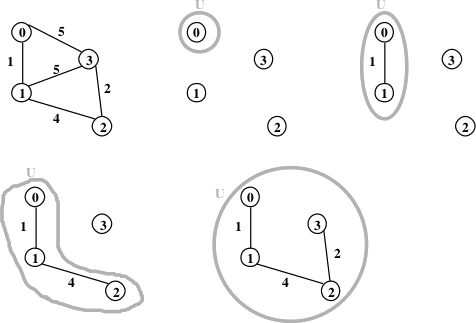
\includegraphics[scale=0.5]{img/ejecuccion_prim}
	\caption{Ejecucción del algoritmo Prim.}
	\label{contexto:figura}
\end{figure}

Al final, el árbol de expansión construido será mínimo. Si el gráfico no estaba conectado originalmente, entonces no existe un árbol de expansión, por lo que el número de aristas seleccionadas será menor que $n-1$.

Lo siguiente es un pseudocódigo del algoritmo que utiliza como estructura de datos auxiliar una cola com prioridad la cual se puede implementar con un heap

\begin{lstlisting}[language=C++]
Prim (Grafo G)
   /* Inicializamos todos los nodos del grafo. 
   La distancia la ponemos a infinito y el padre de cada nodo a NULL
   Encolamos, en una cola de prioridad donde la prioridad es la distancia, 
   todas las parejas <nodo,distancia> del grafo*/
   Por cada u en V[G] hacer
      distancia[u] = INFINITO
      padre[u] = NULL
      Adicionar(cola,<u,distancia[u]>)
   distancia[u]=0
   Mientras !esta_vacia(cola) hacer
	/* OJO: Se entiende por mayor prioridad aquel nodo cuya distancia[u] es menor.*/
      u = extraer_minimo(cola) //devuelve el minimo y lo elimina de la cola.
      Por cada v adyacente a 'u' hacer
         si ((v pertenece cola) && (distancia[v] > peso(u, v)) entonces
            padre[v] = u
            distancia[v] = peso(u, v)
            Actualizar(cola,<v,distancia[v]>)
\end{lstlisting} 

La complejidad del algoritmo depende de cómo busquemos la siguiente arista mínima entre las aristas apropiadas. Hay múltiples enfoques que conducen a diferentes complejidades y diferentes implementaciones.

\subsection{Solución trivial}
Si buscamos la arista iterando sobre todas las aristas posibles, entonces toma $O(m)$ tiempo para encontrar la arista con el mínimo peso. La complejidad total será $O(nm)$. En el peor de los casos esto es $O(n^3)$, realmente lento.

Este algoritmo se puede mejorar si solo miramos un borde de cada vértice ya 
seleccionado. Por ejemplo, podemos clasificar las aristas de cada vértice en 
orden ascendente de sus pesos y almacenar un puntero en la primera arista válida 
(es decir, una arista que va a un vértice no seleccionado). Luego, después de 
encontrar y seleccionar el borde mínimo, actualizamos los punteros. Esto da una 
complejidad de $O(n^2 + m)$ , y para ordenar los bordes un adicional
$O(m \log n)$, lo que da la complejidad $O(n^2 \log n)$ En el peor de los casos.

A continuación, consideramos dos algoritmos ligeramente diferentes, uno para gráficos densos y otro para gráficos dispersos, ambos con una mayor complejidad.


\subsection{Grafos densos}

Abordamos este problema desde un ángulo diferente: para cada vértice aún no seleccionado almacenaremos el borde mínimo en un vértice ya seleccionado. Luego, durante un paso, solo tenemos que mirar estos bordes de peso mínimo, que tendrán una complejidad de $O(n)$. Después de agregar un borde, se deben volver a calcular algunos punteros de borde mínimos. Tenga en cuenta que los pesos solo pueden disminuir, es decir, el borde de peso mínimo de cada vértice aún no seleccionado puede permanecer igual, o se actualizará por un borde al vértice recién seleccionado. Por lo tanto, esta fase también se puede hacer en $O(n)$.

\subsection{Grafos dispersos}

En el algoritmo descrito anteriormente es posible interpretar las operaciones de encontrar el mínimo y modificar algunos valores como operaciones de conjunto. Estas dos operaciones clásicas son compatibles con muchas estructuras de datos, por ejemplo, \emph{set} en C ++ (que se implementan a través de árboles rojo-negro).

El algoritmo principal sigue siendo el mismo, pero ahora podemos encontrar la arista mínimo en $O(\log n)$ tiempo. Por otro lado, volver a calcular los punteros ahora tomará $O(n\log n)$ tiempo, que es peor que en el algoritmo anterior.

